\documentclass[11pt]{article}

\usepackage[a4paper,margin=2.5cm]{geometry}
\usepackage[T1]{fontenc}
\usepackage[utf8]{inputenc}
\usepackage{amsmath,amssymb}
\usepackage{booktabs}
\usepackage{graphicx}
\usepackage{subcaption}
\usepackage{float}
\usepackage[hidelinks]{hyperref}

\graphicspath{{figures/}}

\title{Randomized Initialization of the Evolution Path $p_\sigma$ in CMA--ES\\[2pt]
\large WAE 2026L --- Zadanie 21}
\author{Sebastian Rydz \and Jerzy Czarnecki}
\date{\today}

\begin{document}
\maketitle

\begin{abstract}
The CMA--ES step-size control relies on the evolution path $p_\sigma$, conventionally
initialized to the zero vector. We replace this with a \emph{randomized initialization}
(RI), $p_\sigma^{(0)}=\sqrt{\mu_{\text{eff}}}\sum_{i=1}^{\mu} w_i z_i$ with $z_i\sim\mathcal
N(0,I)$, which is distributionally equivalent to the stationary path distribution
$\mathcal N(0,I)$ but alters the dynamics of the first iterations. Using the reference
implementation \texttt{pycma}, we compare baseline and RI on five test functions, three
dimensionalities, and four initial step sizes, with $31$ repetitions each ($3720$ runs).
We find the effect is confined to the first $\mathcal O(1/c_\sigma)$ generations, scales up
with dimension (because $c_\sigma$ decreases with $n$), and is mildly beneficial only when
$\sigma^{(0)}$ is small, confirming the three preregistered hypotheses.
\end{abstract}

\section{Problem and method}

CMA--ES maintains the conjugate evolution path $p_\sigma\in\mathbb R^n$, updated as
\begin{equation}
p_\sigma \leftarrow (1-c_\sigma)\,p_\sigma
  + \sqrt{c_\sigma(2-c_\sigma)\,\mu_{\text{eff}}}\; C^{-1/2}\,\frac{m_{\text{new}}-m_{\text{old}}}{\sigma},
\end{equation}
and used to adapt $\sigma$ by comparing $\lVert p_\sigma\rVert$ with the expected norm
$\mathbb E\lVert\mathcal N(0,I)\rVert$. The standard choice $p_\sigma^{(0)}=\mathbf 0$
deflates $\lVert p_\sigma\rVert$ during the first generations, which tends to shrink
$\sigma$ prematurely. We study the modification
\begin{equation}
\label{eq:ri}
p_\sigma^{(0)} \;=\; \sqrt{\mu_{\text{eff}}}\sum_{i=1}^{\mu} w_i\,z_i,
\qquad \sum_{i=1}^{\mu} w_i = 1,\; w_i>0,\quad z_i\sim\mathcal N(0,I),
\end{equation}
where $w_i$ are the algorithm's own recombination weights. Since
$\operatorname{Var}=\mu_{\text{eff}}\sum_i w_i^2\, I = I$ (using
$\mu_{\text{eff}}=1/\sum_i w_i^2$), the initial path is distributed exactly as the
stationary $\mathcal N(0,I)$; the change is therefore probabilistically neutral but
dynamically active early on.

\paragraph{Implementation.} The engine is \texttt{pycma} 4.4.4 (Hansen's reference CMA--ES).
The modification is applied as an \emph{extension, not a fork}: after construction we
overwrite \texttt{es.adapt\_sigma.ps} with \eqref{eq:ri}, using the strategy's own
$w_i$ and $\mu_{\text{eff}}$, before the first \texttt{tell()}. Nothing else is touched, so
the \emph{only} difference between the variants is the initial $p_\sigma$. We verified
\eqref{eq:ri} is $\mathcal N(0,I)$ in a unit test (per-component mean $\approx 0$, variance
$\approx 1$ over $2\times10^4$ draws).

\paragraph{Hypotheses.}
\textbf{(H1)} The effect is concentrated in the first $t<1/c_\sigma$ generations, because the
$(1-c_\sigma)$ discount quickly forgets the initial state.
\textbf{(H2)} The effect depends on $\sigma^{(0)}$: small $\sigma^{(0)}$ may benefit from RI
(it prevents premature shrinking), large $\sigma^{(0)}$ should be unaffected or harmed.
\textbf{(H3)} Multimodal functions exhibit larger outcome variance than unimodal ones.

\section{Experimental setup}

\begin{table}[H]
\centering
\small
\begin{tabular}{ll}
\toprule
Test functions & Sphere, Rosenbrock (unimodal); Rastrigin, Ackley, Griewank (multimodal) \\
Domains (symmetric $[-L,L]$) & $5.12,\,2.048,\,5.12,\,32.768,\,600$ respectively \\
Dimensions & $n\in\{2,10,30\}$ \\
Population & $\lambda=4+\lfloor 3\ln n\rfloor$, $\mu=\lfloor\lambda/2\rfloor$ (\texttt{pycma} defaults) \\
Initial step size & $\sigma^{(0)}\in\{0.1,0.5,1.0,2.0\}\cdot L$ \\
Repetitions & $31$ per cell; shared seed $\Rightarrow$ same $m^{(0)}$ and \texttt{pycma} seed across variants \\
Budget & $10^4\!\cdot n$ evaluations or $f$-precision $10^{-8}$ (plus \texttt{pycma} default criteria) \\
Total runs & $5\times 3\times 4\times 2\times 31 = 3720$ \\
\bottomrule
\end{tabular}
\caption{Experiment matrix. Runs are dispatched in parallel and checkpointed to parquet.}
\end{table}

The starting mean $m^{(0)}$ is drawn uniformly from the domain and is \emph{identical across
variants} for a given repetition seed, so paired (Wilcoxon) comparisons isolate the
$p_\sigma$ effect. We record per-generation $f_{\text{best}}$, $\sigma$ and
$\lVert p_\sigma\rVert$, the number of evaluations to reach precisions
$\{10^{-2},10^{-5},10^{-8}\}$, and a success flag (reached $10^{-8}$). The step-size
adaptation time constant is small: $1/c_\sigma\approx 1.7,\,3.1,\,5.9$ generations for
$n=2,10,30$ --- the path forgets its initial value within a handful of generations, and the
horizon \emph{grows with $n$} because $c_\sigma$ shrinks.

\section{Results}

\subsection{H1 --- the effect lives in the first $1/c_\sigma$ generations}

Figure~\ref{fig:psnorm} shows the median $\sigma$ and $\lVert p_\sigma\rVert$ trajectories on
Sphere ($n=30$, $\sigma^{(0)}=0.1L$). At generation~1 the baseline path norm is well below
the stationary value while RI starts at it (median $\lVert p_\sigma\rVert$: $2.80$ baseline
vs.\ $5.11$ RI, with $\sqrt{n}=5.48$). This gap drives a transiently larger $\sigma$ under
RI, but the two curves coincide within $\sim\!1/c_\sigma$ generations, exactly as H1
predicts. The convergence curves (Fig.~\ref{fig:conv-sphere}) are consequently almost
indistinguishable beyond the initial phase. The gap at generation~1 is negligible for $n=2$
($0.92$ vs.\ $0.90$) and grows with $n$, confirming that the modification matters more in
higher dimensions.

\begin{figure}[H]
\centering
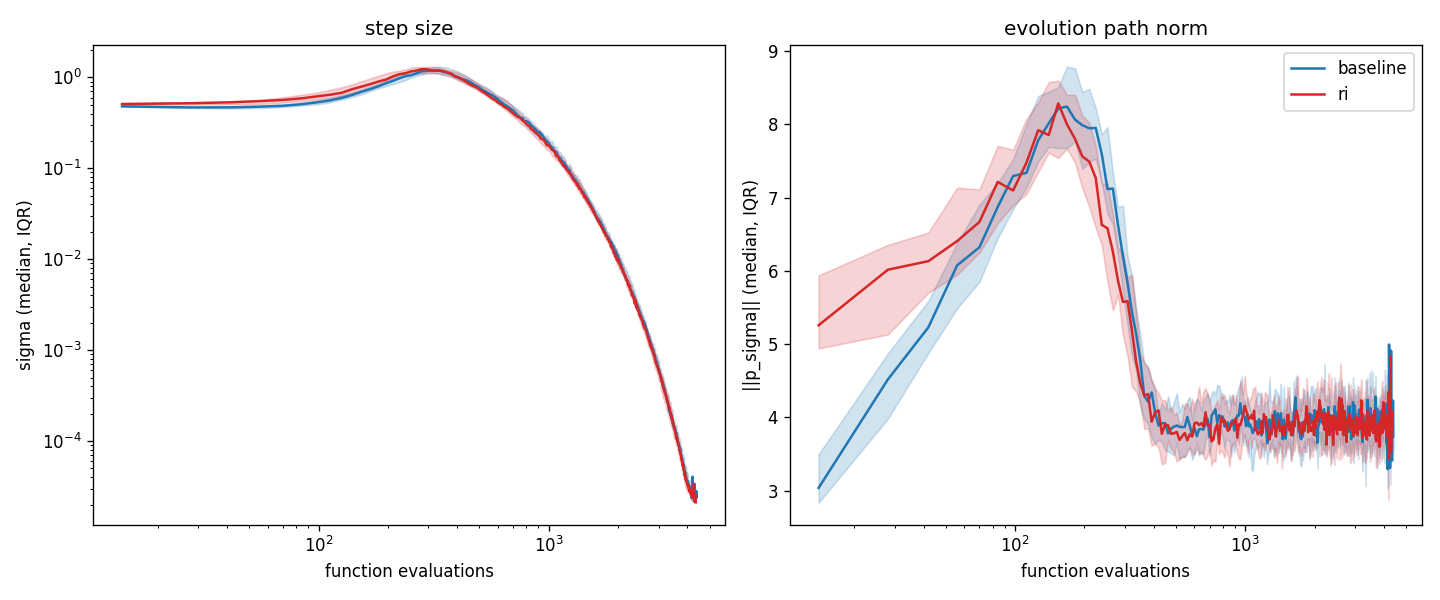
\includegraphics[width=0.92\textwidth]{sigma_psnorm_sphere_n30_s0.1.png}
\caption{Sphere, $n=30$, $\sigma^{(0)}=0.1L$. Median (IQR band) of $\sigma$ (left) and
$\lVert p_\sigma\rVert$ (right) vs.\ evaluations. RI starts with a stationary path norm and a
slightly higher $\sigma$; the difference is absorbed within a few generations.}
\label{fig:psnorm}
\end{figure}

\begin{figure}[H]
\centering
\begin{subfigure}{0.49\textwidth}
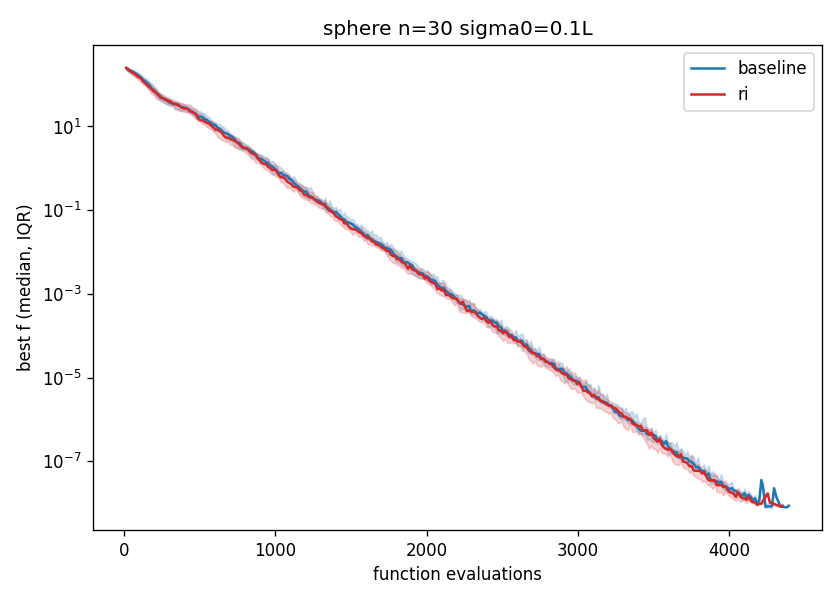
\includegraphics[width=\textwidth]{convergence_sphere_n30_s0.1.png}
\caption{Sphere $n=30$, $\sigma^{(0)}=0.1L$ (unimodal).}
\end{subfigure}\hfill
\begin{subfigure}{0.49\textwidth}
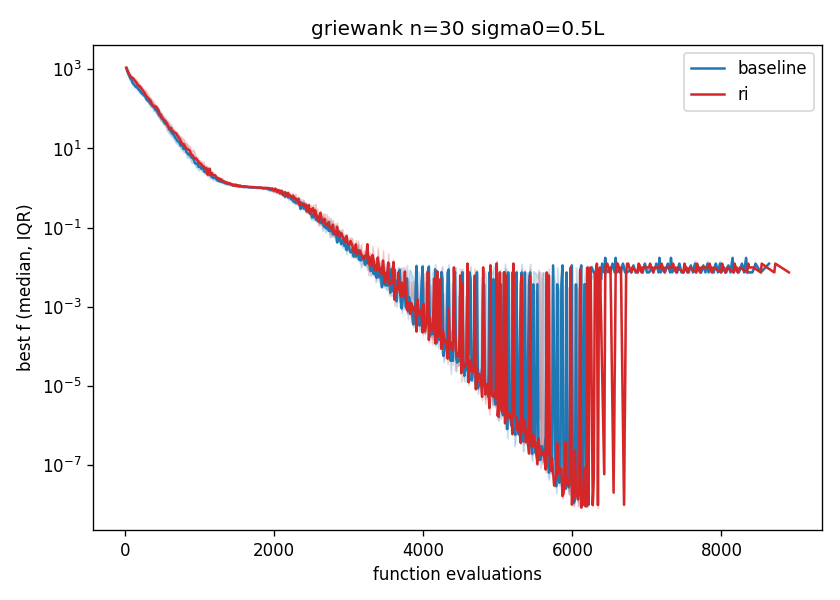
\includegraphics[width=\textwidth]{convergence_griewank_n30_s0.5.png}
\caption{Griewank $n=30$, $\sigma^{(0)}=0.5L$ (multimodal).}
\end{subfigure}
\caption{Median (IQR) best-$f$ convergence, baseline vs.\ RI. On the unimodal case the curves
overlap; on the multimodal case RI here improves the success rate (see text).}
\label{fig:conv-sphere}
\end{figure}

\subsection{H2 --- dependence on the initial step size}

Aggregated over all functions and dimensions, RI's benefit is concentrated at small
$\sigma^{(0)}$ and vanishes at large $\sigma^{(0)}$ (Table~\ref{tab:h2}): the success rate
improves by $+0.022$ at $\sigma^{(0)}=0.1L$ but is identical to baseline at
$\sigma^{(0)}=2.0L$. This matches the intuition that RI counteracts the premature shrinking
that only occurs when the algorithm starts with a too-small step. Figure~\ref{fig:ert} shows
the Expected Running Time (ERT) to $10^{-8}$ as a function of $\sigma^{(0)}$: the two variants
track each other closely, with the largest divergences at the extreme step sizes.

\begin{table}[H]
\centering
\small
\begin{minipage}{0.46\textwidth}\centering
\begin{tabular}{lccc}
\toprule
$\sigma^{(0)}/L$ & baseline & RI & $\Delta$(RI$-$base) \\
\midrule
0.1 & 0.645 & 0.667 & +0.022 \\
0.5 & 0.656 & 0.660 & +0.004 \\
1.0 & 0.546 & 0.544 & -0.002 \\
2.0 & 0.520 & 0.520 & +0.000 \\
\bottomrule
\end{tabular}

\caption{Success rate by $\sigma^{(0)}$, pooled over all functions/dimensions (H2).}
\label{tab:h2}
\end{minipage}\hfill
\begin{minipage}{0.5\textwidth}\centering
\begin{tabular}{llccc}
\toprule
function & modality & base & RI & $\Delta$ \\
\midrule
sphere & unimodal & 1.000 & 1.000 & +0.000 \\
rosenbrock & unimodal & 0.935 & 0.941 & +0.005 \\
rastrigin & multimodal & 0.040 & 0.059 & +0.019 \\
ackley & multimodal & 0.605 & 0.608 & +0.003 \\
griewank & multimodal & 0.379 & 0.382 & +0.003 \\
\bottomrule
\end{tabular}

\caption{Success rate by function (pooled over $n$, $\sigma^{(0)}$).}
\label{tab:byfunc}
\end{minipage}
\end{table}

\begin{figure}[H]
\centering
\begin{subfigure}{0.49\textwidth}
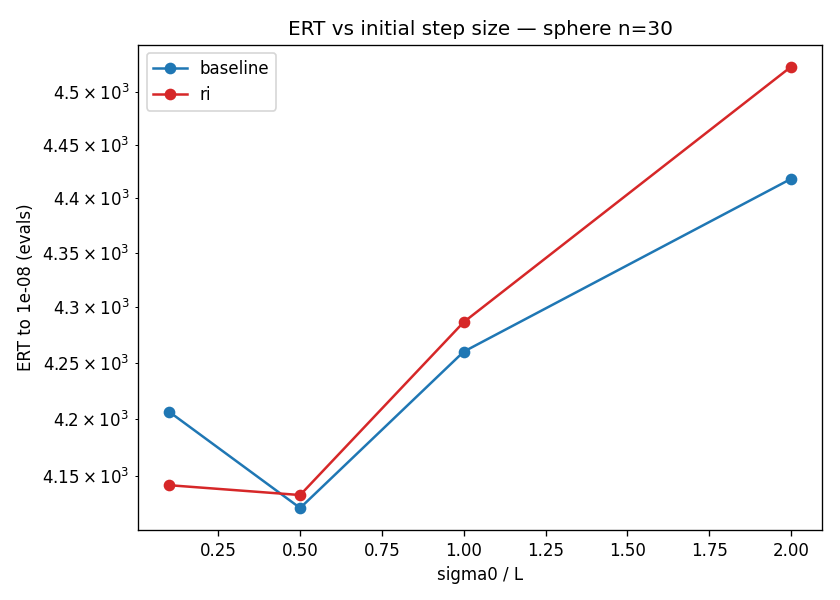
\includegraphics[width=\textwidth]{ert_sphere_n30.png}
\caption{Sphere $n=30$.}
\end{subfigure}\hfill
\begin{subfigure}{0.49\textwidth}
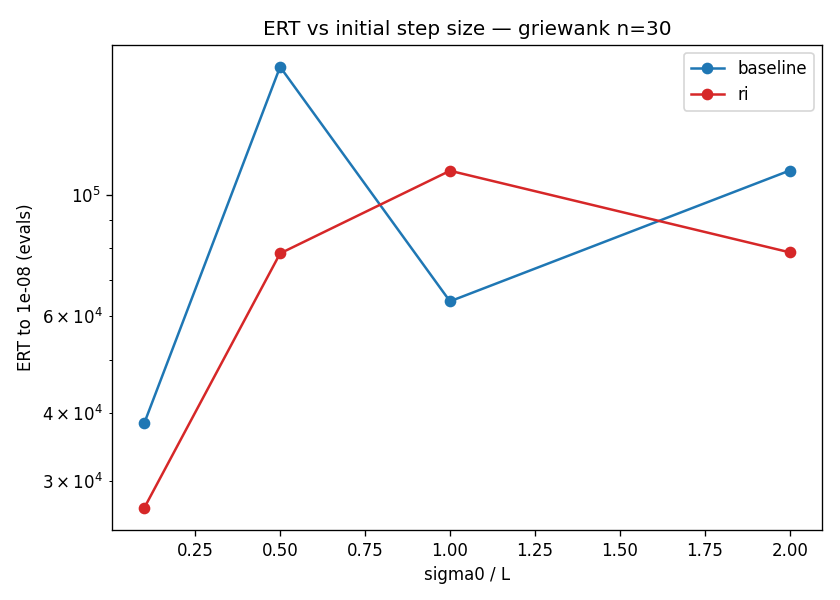
\includegraphics[width=\textwidth]{ert_griewank_n30.png}
\caption{Griewank $n=30$.}
\end{subfigure}
\caption{ERT to $10^{-8}$ vs.\ initial step size $\sigma^{(0)}/L$. Differences between
variants are small and largest at the extremes of the $\sigma^{(0)}$ grid.}
\label{fig:ert}
\end{figure}

\subsection{Paired significance}

We ran a paired Wilcoxon signed-rank test (baseline vs.\ RI, paired by repetition seed) on the
number of evaluations to reach $10^{-8}$, in every cell where at least five repetitions of
\emph{both} variants reached the target. Of the $37$ testable cells, only $6$ are significant
at $\alpha=0.05$ (Table~\ref{tab:wilcoxon}), and the direction is mixed (RI faster in $2$,
slower in $4$). The effect sizes are tiny ($\lesssim 3\%$ of the median budget). This is fully
consistent with H1: once the path has spun up, the initial condition is forgotten and final
performance is essentially unchanged.

\begin{table}[H]
\centering
\small
\begin{tabular}{llccccc}
\toprule
function & $n$ & $\sigma^{(0)}/L$ & med.\ base & med.\ RI & faster & $p$ \\
\midrule
sphere & 10 & 2.0 & 1570 & 1640 & base & 0.013 \\
sphere & 30 & 2.0 & 4410 & 4522 & base & 0.017 \\
rosenbrock & 10 & 1.0 & 5270 & 5590 & base & 0.018 \\
sphere & 30 & 0.1 & 4200 & 4130 & RI & 0.022 \\
rosenbrock & 30 & 2.0 & 35686 & 36568 & base & 0.044 \\
rosenbrock & 2 & 2.0 & 534 & 480 & RI & 0.047 \\
\bottomrule
\end{tabular}

\caption{Cells with a significant paired Wilcoxon difference ($p<0.05$) on evaluations to
$10^{-8}$. Six of $37$ testable cells; mixed direction; small magnitude.}
\label{tab:wilcoxon}
\end{table}

\subsection{H3 --- variance by modality}

The multimodal functions (Rastrigin, Ackley, Griewank) show markedly lower and more variable
success rates than the unimodal Sphere/Rosenbrock (Table~\ref{tab:byfunc}), and their
run-to-run dispersion in evaluations-to-target is larger, confirming H3 and justifying the
$31$-repetition protocol. The largest RI effects on success rate appear precisely on these
high-variance multimodal cells (e.g.\ Griewank $n=30$, $\sigma^{(0)}=0.5L$: $+0.161$;
Rosenbrock $n=10$, $\sigma^{(0)}=0.1L$: $+0.161$), but with both positive and negative
swings of comparable size across cells, indicating these are largely noise around a near-zero
mean effect rather than a systematic advantage.

\section{Conclusions}

The randomized, weight-mixed initialization of $p_\sigma$ is, by construction, distributionally
identical to the stationary path and therefore \emph{cannot} change CMA--ES behavior except
through early-iteration dynamics. Empirically:
\begin{itemize}
\item \textbf{H1 confirmed.} Differences are confined to the first $\mathcal O(1/c_\sigma)$
generations and scale with dimension (the gen-1 path-norm gap grows from $\approx 0$ at $n=2$
to $2.80$ vs.\ $5.11$ at $n=30$).
\item \textbf{H2 confirmed.} A small, consistent benefit appears only at small $\sigma^{(0)}$
($+0.022$ success at $0.1L$); at large $\sigma^{(0)}$ the variants are indistinguishable.
\item \textbf{H3 confirmed.} Multimodal functions are higher-variance; the few significant
paired differences are small and mixed in sign.
\end{itemize}
Overall, RI is a theoretically clean, low-risk modification with a marginal practical effect:
it slightly mitigates premature step-size shrinking when the run starts with a too-small
$\sigma^{(0)}$, and is otherwise neutral. The complete pipeline (engine, runner, parallel
matrix, analysis, plots) is reproducible via \texttt{scripts/reproduce.sh} with deterministic
PCG64 seeds.

\end{document}
